\chapter{Návrh a implementace rozšíření} \label{5Chapter}
Rozšíření bude implementováno v jazyce Typescript. K vytvoření rozšíření samotného je potřeba Node.js \cite{nodejs} a Git \cite{git}. Poté je vyžadována instalace programů Yeoman \cite{yeoman} a VS Code Extension Generator \cite{YO_Generator}, pomocí kterých jsou rozšíření generovány.\\

\section{Třída extension.ts}
Základní třída, která je součástí každého VS Code rozšíření, je třída \textbf{extension.ts}. Na začátku třída obsahuje pouze jedinou funkci, a to \textit{function activate(context: vscode.ExtensionContext)}. Tato Funkce rozšíření aktivuje, pokud narazí na soubor s příponou \textbf{.mc}. Seznam přípon souborů, při jejich otevření se rozšíření aktivuje, je uveden v konfiguračním package.json souboru, viz \ref{src:activation}. Rozšíření se také aktivuje v případě, že pracovní adresář obsahuje Monkey C soubor. V package.json souboru jsou mimo jiné uvedeny informace, jako název rozšíření, jeho popis, autor, aktuální verze, atd...\\

\begin{lstlisting}[language=Python,label=src:activation,caption={aktivační události rozšíření}]
        "activationEvents": [
			"onLanguage:monkeyc",
			"workspaceContains:.mc"
		]
\end{lstlisting}

Funkce \textit{\textbf{activate()}} přijímá parametr context. Tento parametr reprezentuje nástroje, se kterými rozšíření pracuje. Tělo funkce se skládá z několika podpůrných tříd, tzv. providerů. Providery jsou součástí VS Code API (jedná se o sadu JavaScript rozhraní, které mohou být vyvolány rozšířením) \cite{vscodeAPI}. \\
První provider ve třídě extension zajišťuje obarvování Monkey C syntaxe, viz. \ref{sec:obarveni_kodu}. Dále následuje funkce \textit{onDidOpenTextDocument()}. Jedná se o událost, která se vyvolá při otevření textového dokumentu. Zde je také řešeno parsování souborů. Pokud uživatel otevře pracovní adresář, tedy složku, která obsahuje více soborů, spustí se funkce parseAllDocuments(). Událost \textit{onDidChangeTextDocument()} společně s funkcí parseCurrentDocument() dále řeší parsování aktuálně upravovaného dokumentu, a to vždy když dojde k nějaké změně. Dále třída extension.ts obsahuje sadu providerů, které zajišťují našeptávání a dokončování kódu \ref{src:completionProvider}. Tento provider přijímá následující tři parametry: 

\begin{enumerate}
\item \textbf{selector} - definuje dokumenty, na které má být provider aplikován
\item \textbf{provider} - definuje konkrétní provider
\item \textbf{...triggerCharacters} - jedná se o pole znaků, při kterých má být provider aktivován. V rozšíření jsou pro aktivaci providerů nejčastěji použity symboly tečky a mezery
\end{enumerate}

\textbf{keywordsProvider} - Provider zajišťující našeptávání klíčových slov jazyka. Pro získání vhodných klíčových slov je použit c3 Engine, popsán v sekci \ref{55section}\\

\textbf{importedModulesProvider} - Pokud jsou ve zdrojovém kódu programu, prostřednictvím klíčového slova \textbf{using}, importovány nějaké moduly, tento provider vrátí jejich seznam. V následujícím výpisu kódu je importováno 5 modulů a 1 třída z Toyboxu. Seznam který provider vrátí bude tedy obsahovat 5 názvů modulů a 1 název třídy [WatchUi, Graphics, System, Lang, Object, Time], kde Object je název třídy. V tomto seznamu jsou hodnoty uloženy jako \textbf{vscode.CompletionItem} \ref{img:CompletionItem}. Jedná se o třídu, která je součástí VS Code API. Její konstruktor přijímá 2 parametry, název položky a její druh. Druh položky, CompletionItemKind, představuje výčet, který obsahuje prvky, jako modul, třída, proměnná, funkce, konstanta, atd...\\


\begin{lstlisting}[language=Python,label=src:usingStatements,caption={importované moduly z Toyboxu}]
      using Toybox.WatchUi;
		using Toybox.Graphics;
		using Toybox.System;
		using Toybox.Lang;
		using Toybox.Lang.Object;
		using Toybox.Time;
\end{lstlisting}



\begin{lstlisting}[language=Python,label=src:completionProvider,caption={aktivační události rozšíření}]
        registerCompletionItemProvider(selector: DocumentSelector, provider: CompletionItemProvider, ...triggerCharacters: string[]): Disposable
\end{lstlisting}

\textbf{localVariableProvider} , \textbf{classVariableProvider} -Providery zajišťující našeptávání lokálních proměnných ve zdrojovém kódu. V Monkey C existují 2 způsoby, jak lze přistupovat k proměnným. Pokud se jedná o vnitřní proměnnou třídy, přístup k ní není nijak omezen. Pokud je proměnná označena jako \textbf{public} nebo \textbf{protected}, je potřeba k ní přistoupit pomocí prefixů \textbf{self.} nebo \textbf{me.}.\\

\begin{figure}
	\centering
	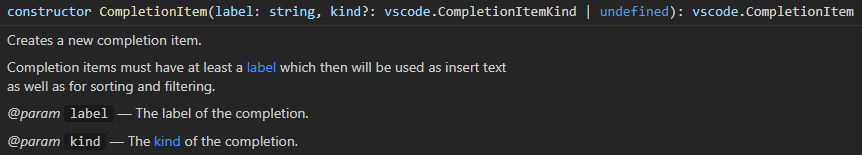
\includegraphics[width=\textwidth,scale=1]{images/CompletionItem}
	\caption{popis konstruktoru třídy CompletionItem z VS Code API}
	\label{img:CompletionItem}
\end{figure}

\textbf{functionProvider} - Provider pro funkce ve zdrojovém kódu. Výše bylo zmíněno, že každá funkce musí být před použitím deklarována a nelze ji předat přímo, jako parametr jiné funkci. Pokud však použijeme funkci \textbf{method()} z třídy Toybox.Lang.Object, instance této třídy dokáže vytvořit objekt třídy Toybox.Lang.Method, díky které je tuto funkci vyvolat, jako callback, viz. výpis kódu \ref{src:callback}.\\

\textbf{toyboxProvider} - slouží pro našeptávání komponent Toyboxu při importování do aplikace, např. modulů a tříd, viz. výpis kódu \ref{src:usingStatements}. Pro získání modulů je použita funkce \textit{findModuleBodyMembers()}, která prochází syntaktickém strom a hledá uzel, ve kterém je uložen Toybox. Jelikož je tento modul rodičem pro všechny ostatní moduly, stačí nalézt první uzel, který obsahuje pravidlo \textit{$MonkeyCParser.RULE_moduleBodyMembers$}, viz. výpis kódu \ref{src:findModuleBodyMembers}. Následně stačí pomocí metody \textbf{getChildren()} získat všechny jeho potomky. Z těchto potomků poté funkce \textbf{collectClassesFromModules()} získá názvy všech tříd, které je možné importovat.\\

\begin{lstlisting}[language=Python,label=src:callback,caption={ukázka použití funkce, jako callback}]
    //! Constructor
    function initialize()
    {
        View.initialize();
        Sensor.enableSensorEvents( method(:onSnsr) );

    }

    function onSnsr(sensor_info)
    {
        //function body
    }
\end{lstlisting}

\begin{lstlisting}[language=Python,label=src:findModuleBodyMembers,caption={funkce prochází strom a hledá uzel, ve kterém je uložen Toybox}]
                    if(tree[i].getContext()!?.ruleIndex === MonkeyCParser.RULE_moduleBodyMembers) {
                    modules = tree[i].getChildren()!;
                    break;
                }
\end{lstlisting}

\textbf{accessibleMembersProvider} - Tento provider zajišťuje především našeptávání na proměnných nějakého typu, jak je možné vidět na obrázku \ref{img:autocomplete_example}, kde rozšíření našeptává metody z třídy Toybox.Lang.String. Pokud je tedy proměnná například instance třídy, nebo se jedná o importovaný modul, provider podle toho v syntaktickém stromě nalezne, co se pod daným identifikátorem nachází, a podle toho jsou volány příslušné funkce. Například pro nalezení všech přístupných členů instance třídy je použita funkce \textbf{collectAccessibleMembers()}.\\

\textbf{inheritedMembersProvider} - Jsou deklarovány třídy \textbf{A} a \textbf{B}, kde třída \textbf{B} je potomkem třídy \textbf{A}. V Monkey C je dědičnost podporována a k její identifikaci je použito klíčové slovo \textbf{extends}. V tomto případě by tedy deklarace třídy B vypadala \textit{class B extends A {}}. Pokud chceme přistoupit ke členům rodičovské třídy A, provede tento provider příslušné operace a vrátí seznam dostupných členů.\\

\textbf{importedMembersProvider} - Tento provider se stará o našeptávání tříd z importovaných modulů. Na obrázku \ref{img:importedModules} lze vidět, jak rozšíření našeptává prvních 5 tříd z importovaného modulu Toybox.Application. Provider je aktivován, pokud se na řádku nachází klíčové slovo \textbf{new}, tím pádem pozná, že chce uživatel vytvořit novou instanci třídy.\\


\begin{figure}[b!]
	\centering
	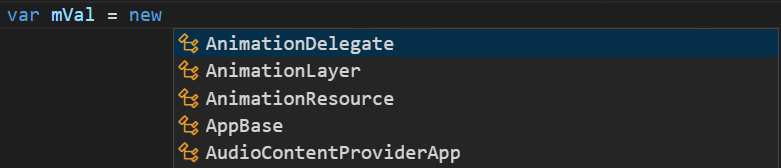
\includegraphics[width=\textwidth,scale=1]{images/importedModules}
	\caption{rozšíření našeptává třídy z importovaných modulů.}
	\label{img:importedModules}
\end{figure}

\textbf{curlyBracesProvider}, \textbf{normalBracesProvider} - Zde bylo záměrem automaticky do dokumentu doplnit pravou závorku po zadání levé. Například v situaci, kdy uživatel napíše levou závorku '\textbf{$($}', rozšíření automaticky do textu doplní druhou. Doplnit takto závorku do dokumentu se však nepodařilo. Místo toho provider uživateli závorku navrhne, stejně jako navrhují kandidáty ostatní providery, a ten ji následně po stisknutí tlačítka tab na klávesnici doplní.\\

\textbf{multilineCommentProvider} - Tento provider zajišťuje našeptávání 2 typů víceřádkových komentářů. První typ je klasický prázdný víceřádkový komentář, který nalezneme ve většině programovacích jazyků. Druhý typ, který je možné vidět na obrázku \ref{img:comments}, je specifický tím, že v sobě obsahuje \textbf{@type}. Tento komentář slouží k popisu proměnné při její deklaraci. Za prefix  \textbf{@type} uživatel uvede datový typ proměnné. Je zde využito toho, že v Monkey C musí být proměnná před použitím deklarována, jak už zde bylo několikrát zmíněno a jak je popsáno v sekci \ref{55section}.\\

\textbf{dataTypesProvider} - Další a zároveň poslední provider ve třídě \textbf{extension.ts}, který úzce souvisí s providerem předchozím, je dataTypesProvider. Jak už je z názvu patrné, provider zajišťuje našeptávání všech datových typů z Toyboxu. Na obrázku \ref{img:data_types} lze vidět, jak rozšíření našeptává datové typy z Toyboxu.\\

\begin{figure}[h!]
	\centering
	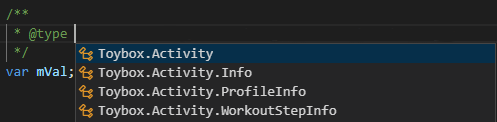
\includegraphics[width=\textwidth,scale=1]{images/data_types}
	\caption{rozšíření našeptává datové typy z modulu Toybox.Activity.}
	\label{img:data_types}
\end{figure}

Na začátku této sekce byla zmíněna funkce \textit{activate()}, která je volána při spuštění rozšíření. K ní je, jako protiklad, na konci funkce \textit{deactivate()}, která je volána v momentě, kdy je deaktivováno rozšíření.\\

\section{Třída documentHandler.ts}
Jedná se o jednu z nejdůležitějších a nejrozsáhlejších tříd v celé aplikaci. Obsahuje přes 30 metod, které zajišťují plynulý chod rozšíření. Nacházejí se zde Mapy, ve kterých jsou uloženy veškeré informace jednotlivých dokumentů, jak je popsáno v sekci \ref{44SemantickaAnalyza}. Nejdůležitějšími třídami jsou však \textit{\textbf{parseAllDocuments()}} a \textit{\textbf{parseCurrentDocument()}}. Funkce \textit{\textbf{parseAllDocuments()}} je při aktivaci rozšíření volána jako první. Zde dochází k načtení všech souborů z pracovního adresáře. Následně je pro daný soubor vytvořen \textit{inputStream}, jenž je jako parametr předán instanci \textbf{MonkeyCLexer}u. Dále dojde k vytvoření \textbf{tokenStream}u, jenž je předán instanci \textbf{MonkeyCParser}u. Poté dojde k parsování dokumentu a vytvoření syntaktického stromu jak pro zdrojový kód, tak pro komentáře, viz. obrázek \ref{img:parsing_input}.\\


\begin{figure}[]
	\centering
	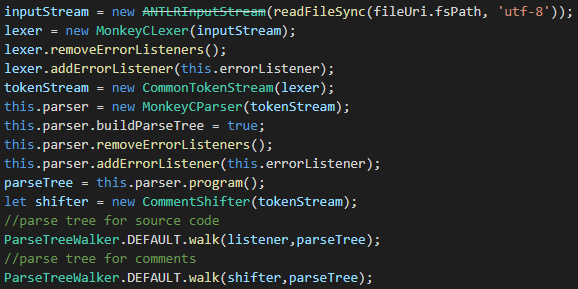
\includegraphics[width=\textwidth,scale=1]{images/parsing_input}
	\caption{vytvoření instancí parseru a lexeru a následné parsování soboru.}
	\label{img:parsing_input}
\end{figure}

Dále je volána funkce \textbf{provideAutocomplete()}, která ze syntaktické stromu získá proměnné, funkce, atd... Vždy pro konkrétní dokument. Funkce updateCollection() poté zpracuje všechny syntaktické chyby, která detekoval Error Listener \ref{errorListener}.\\

Funkce \textit{\textbf{parseCurrentDocument()}} vykonává stejnou činnost, jako výše popsaná pouze s tím rozdílem, že tato funkce je volána vždy při práci s konkrétním dokumentem.

\section{Třída Listener.ts}
Jedná se o třídu, která implentuje rozhraní \textbf{MonkeyCListener}. Toto rozhraní  definuje kompletní listener pro parser vytvořený \textbf{MonkeyCParser}em. jinými slovy, nacházejí se zde všechny metody, které jsou potřeba pro vytvoření syntaktického stromu při průchodu parseru. Příklad vytvořených metod je možné vidět na obrázku \ref{img:listener_functions}. Kromě zpracovávání zdrojového kódu třída Listener zajišťuje také zpracování komentářů. Toto je zajištěno prostřednictvím třídy \textit{CommentShifter}, převzaté z Definitive ANTLR 4 reference \cite{ANTLR_2013}. Tato třída umožňuje přístup ke skrytému kanálu s komentáři, které jsou od zdrojového kódu odděleny.

\section{Error Listener} \label{errorListener}
Třída, která slouží k detekování zachytávání syntaktických chyb v kódu. Jedná se o chyby, které jsou v rozporu z pravidly gramatiky. Každá chyba, kterou rozšíření detekuje, je uložena do struktury \textbf{ErrorDescription} \ref{src:ErrorDescription}. Všechny chyby jsou poté uloženy v poli a pomocí metody getSyntaxErrors() je možné je získat. Rozšíření chyby vypisuje do konzole, jak je ve VS Code zvykem. Součástí zprávy jsou:
\begin{enumerate}
\item řádek, na kterém se chyba nachází
\item pozice na řádku
\item popis chyby
\end{enumerate}

\begin{lstlisting}[language=Python,label=src:ErrorDescription,caption={rozhraní pro popis chyby}]
export interface ErrorDescription {
	document: string;
	offendingSymbol: any;
	line: number;
	charPositionInLine: number;
	msg : string
	e: RecognitionException | undefined
}
\end{lstlisting}

\section{Modul Toybox}
Modul Toybox představuje v Monkey C jmenný prostor (namespace), pod kterým jsou seskupovat třídy, metody, funkce, atd... Obsahuje všechny potřebné třídy, které Monkey C poskytuje, na jednom místě. Z názvů jednotlivých modulů a tříd lze jednoduše odvodit, jaké metody se zde nachází a k jakému účelu slouží.\\ 
Jelikož tento modul, není nikde oficiálně dostupný. Respektive neexistuje žádná oficiální verze, kterou by bylo možné použít, bylo nutné sestavit modul vlastními silami. K jeho vytvoření bylo použito oficiální Connect IQ SDK. V tomto SDK jsou obsaženy informace, ke všem komponentům Toyboxu. Problémem bylo, že zdrojem těchto informací byly soubory ve formátu .html, tedy webové stránky. Bylo tedy nutné veškeré informace extrahovat z html elementů a následně je sestavit do požadované formy. Jelikož bylo vygenerování Toyboxu velmi pracné a extrakce jednotlivých částí z html elementů vyžadovala mnoho úsilí, není zaručeno, že je Toybox zcela kompletní. Vygenerovaný Toybox například neobsahuje deklarované konstanty, které se v některých třídách v oficiální dokumentaci nachází. Velkou výhodou by bylo, kdyby společnost Garmin Ltd. \cite{GARMIN_OFFICIAL} vydala svoji plnohodnotnou verzi Toyboxu. Toto by při vývoji rozšíření ušetřilo velké množství práce a času stráveném při jeho generování.

\section{Obarvení kódu} \label{sec:obarveni_kodu}
Zvýraznění a obarvení Monkey C syntaxe bylo převzato z GitHub repozitáře \cite{syntax_highlight}. Autor Alexander Fedora \cite{fedora} zde k obarvení klíčových slov Monkey C využívá JSON souboru. Tento soubor obsahuje všechna klíčová slova, ty pomocí regulárních výrazů vyhledává v textu a poté je obarvuje.

\begin{figure}
	\centering
	\subfloat[před\label{img:uncolored_code}]
	{
		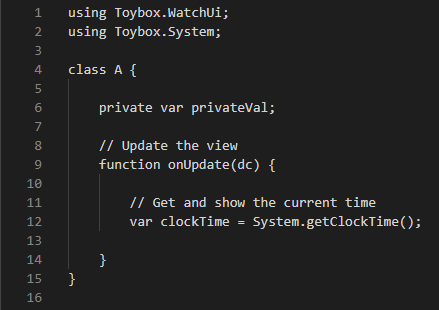
\includegraphics[width=0.45\textwidth]{images/uncolored_code}
	}
	\hspace{1.5em} % make more space
	\subfloat[po\label{img:colored_code}]
	{
		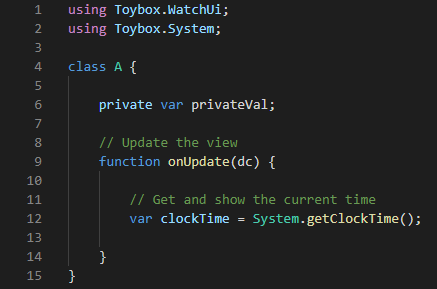
\includegraphics[width=0.45\textwidth]{images/colored_code}
	}
	\caption{Monkey C kód před a po přidaní obarvení syntaxe}
	\label{img:obarveni}
\end{figure}
	
Hned na první pohled je zřejmé, že obarvení poskytuje uživateli větší přehled a orientaci v kódu, jak je vidět na obrázku \ref{img:colored_code}.


\section{Automatické doplňování a našeptávání kódu} \label{55section}
Jako první bylo v rozšíření řešeno našeptávání klíčových slov jazyka, např. NEW, VAR, FUNCTION, atd... k tomuto účelu byl použit "The ANTLR4 Code Completion Core"  \cite{mike_lischke}. Jedná se o "stroj"  sloužící k dokončování kódu pro analyzátory založené na ANTLR4. Engine c3 je schopen poskytnout kandidáty na doplnění kódu, kteří jsou užiteční pro editory s analyzátory generovanými ANTLR, nezávisle na skutečném jazyku / gramatice použité pro generování. Původní implementace je poskytována v jazyce Typescript, což bylo vhodné použít vzhledem k tomu, že rozšíření je také psáno v Typescriptu.
\\
Dále bylo řešeno našeptávání lokálních funkcí a proměnných. V Monkey C jsou k tomuto účelu použity 2 prefixy \textbf{self.} a \textbf{me.}. Pokud uživatel v kódu zadá jeden z těchto prefixů, rozšíření spustí funkci \textbf{provideAutocomplete}, která pomocí průchodu syntaktickým stromem všechny dostupné proměnné, funkce, či třídy, podle toho, kde se zrovna uživatel v kódu nachází.
\\
V neposlední řadě bylo potřeba vyřešit, jak zjistit, co se nachází v konkrétní proměnné, a na základě toho poté provést příslušné našeptávání. Toto je řešeno  pomocí komentářů. Tyto Komentáře se objevují jednak v Toyboxu, kde slouží pro orientaci v už tak rozsáhlém modulu a popisu jednotlivých jeho součástí. Součástí popisu jsou informace o datových typech, vstupních parametrech ( pokud se jedná o funkci), návratových typech atd...  
\\
Komentáře má také k dispozici uživatel přímo v kódu. Každá proměnná, která je deklarována, by měla na sebou obsahovat komentář nesoucí informaci o datovém typu této proměnné. Komentář má jednoduchou syntax, viz. \ref{src:comment}, a rozšíření je navíc schopné jeho stukturu automaticky doplnit po zadání "\textbf{/**}". Je zde využito toho, že každá proměnná v Monkey C musí být deklarována předtím, než ji lze použít. A právě na základě tohoto byly v rozšíření komentáře implementovány. Není tedy potřeba složitě hledat a ukládat informace o datovém typu do nějaké struktury, stačí pouze v kanálu komentářů najít příslušný řádek, na kterém je proměnná deklarována a z něj datový typ extrahovat.

\begin{lstlisting}[language=Python,label=src:comment,caption={struktura komentáře datový typ}]
        /**
         * @type Toybox.Lang.Number
         */
\end{lstlisting}

\begin{figure}[tbh!]
	\centering
	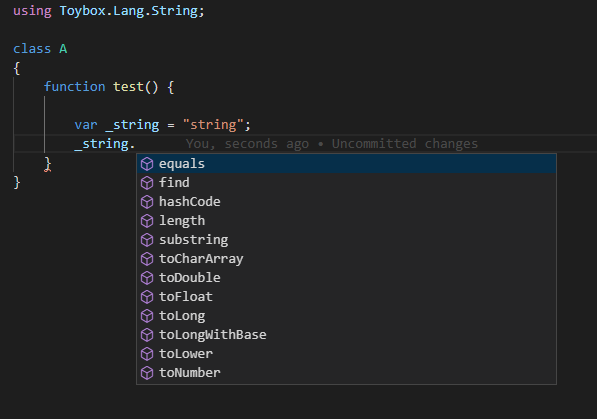
\includegraphics[scale=0.85]{images/autocomplete_example}
	\caption{ukázka automatického našeptávání kódu na proměnné typy string}
	\label{img:autocomplete_example}
\end{figure}

\begin{figure}[b!]
	\centering
	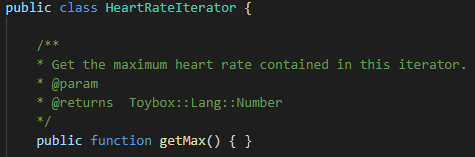
\includegraphics{images/comments}
	\caption{komentář nad funkcí obsahující stručný popis, parametry funkce a návratový typ}
	\label{img:comments}
\end{figure}

\section{Popis funkcí a proměnných Toyboxu}
Rozšíření dokáže při našeptávání jednotlivých částí Toyboxu zobrazit jejich název, druh a popis. A právě k jejich popisu bylo využito komentářů, která každá funkce a proměnná obsahuje. Tyto komentáře vznikly při generování Toyboxu a kromě popisu mají mnoho dalších účelů popsaných výše(např. našeptávání datového typu proměnné).
Na obrázku \ref{img:description} lze vidět popis funkce registerSensorDataListener() z modulu Toybox.Sensor. Součástí popisu je:

\begin{enumerate}
\item návratový typ funkce
\item název funkce
\item popis funkce
\item jednotlivé parametry společně s jejich datovým typem
\end{enumerate}

\begin{figure}[tbh!]
	\centering
	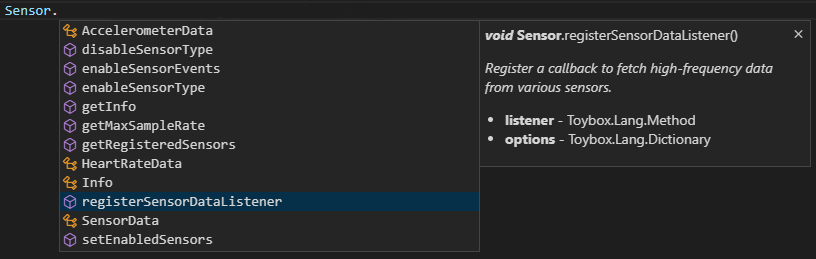
\includegraphics[width=\textwidth,scale=1]{images/description}
	\caption{popis funkce registerSensorDataListener() z modulu Toybox.Sensor.}
	\label{img:description}
\end{figure}


\section{Nedostatky rozšíření}
Při implementaci automatického našeptávání byl detekován problém, kvůli kterému není možné provést volání více funkcí po sobě na jednom řádku. Uveďme si příklad, kdy máme proměnnou typu \textbf{String}, v níž je uloženo číslo. Hodnotu v této proměnné budeme chtít převést na typ Integer, čili zavolat metodu \textit{toNumber()}, a poté bezprostředně po volání \textit{toNumber()} zavolat další metodu. Zde nastává problém, kdy rozšíření, jako další vstup neočekává možné volání funkce \ref{img:autocomplete_errormessage}. Jádrem tohoto problému je, že poskytnutá bezkontextová gramatika popisující jazyk není stoprocentně přesná. A právě kvůli těmto "nepřesnostem" je možné při implementaci narazit na podobné komplikace. V průběhu vývoje zatím nebyly registrovány další problémy způsobené gramatikou.

\begin{figure}[tbh!]
	\centering
	
\includegraphics[scale=1]{images/autocomplete_error}
	\caption{nedostatek rozšíření}
	\label{img:autocomplete_error}
\end{figure}

\begin{figure}[tbh!]
	\centering
	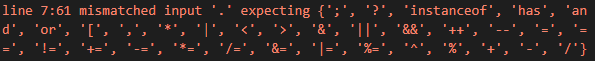
\includegraphics[scale=0.8]{images/autocomplete_errormessage}
	\caption{chybová hláška z error listeneru}
	\label{img:autocomplete_errormessage}
\end{figure}
\endinput